\section{The Git structure}
Git, as it was said before, is a distributed version control system.
It means that each user as a mirror of the repository (local
repository) and in the case of
git, there is no need for a central server, even that, each user is able to
fetch or push updates from other user's repository (remote repository).
Git is divided mainly in three components. The working directory,
the index and the repository. The connection between these components
can be seen in Figure \ref{fig:git_structure}. Local and remote
repository have the same internal structure. What is a local
repository for an user is a remote repository for another user.

\begin{figure}[h!]
   \centering
   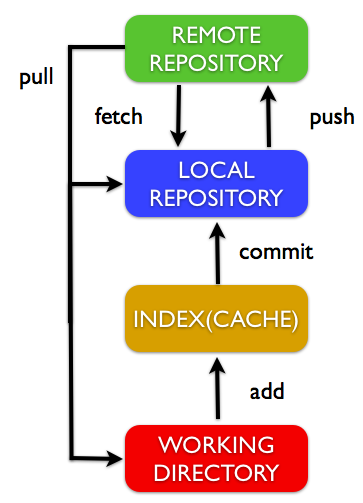
\includegraphics[width=0.8\textwidth]{images/data_flow_simplified.png}
   \caption{Git WorkFlow}\label{fig:git_structure}
\end{figure}

\subsection{Repository}
Git repository is like a database of your system along time. It is
the place where the snapshots taking during the project construction
are kept, as well as, all the necessary information to
allow the users to go through all the snapshots. The snapshot
structure and snapshots relations are kept using what is called \emph{git
objects}. The information needed to go through the project is kept in
what is called \emph{git references}. In the next subsections we
present both of them.

\subsubsection{Git Objects}
As we have presented before git keeps snapshots of how your system
looked like on a certain moment in time. This moment in time is
represented in git by a commit. A commit points to a tree, that
represents the structure of your system on that moment. So a tree
contains others trees and/or blobs. In git the files are not kept. 
What git keeps is a blob that represents the content of files. The
relation between the path of a file and the content of that path 
is kept on the trees corresponding to that path. \par


%git pro 
%You need to make some changes and commit snapshots of those changes into
%your repository each time the
%project reaches a state you want to record.

\subsection{Working Directory}

The working directory is basically a subset of
a file system that contains the files of the project you are
currently working on. This files can be the current files, files
retrieved from an old snapshot or even files that are not being
tracked. When retrieving an older snapshot of the project, the
working directory is updated to reflect the project in that state. It
is possible to have in the working directory files that are not being
tracked. This files are just ignored

\subsection{Index}
The index is a component that contains all the files that will be committed
on the next commit (the next snapshot).

